\section{Introduction to Machine Learning}
\begin{frame}{What is Machine Learning?}
    % Top definition
    \textbf{Machine Learning} is the field of study that gives computers the ability to learn (using data) without being explicitly programmed.
    \vspace{1.5em}

    \begin{columns} % T aligns columns at the top
        % Left Column: Traditional
        \begin{column}{0.48\textwidth}
            \centering            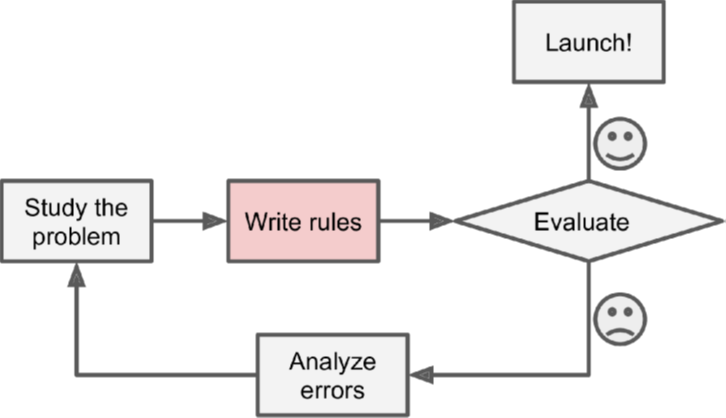
\includegraphics[width=1.0\linewidth]{images/traditional.png} 
            \vspace{1em}
            \textit{The traditional approach} \\
            % \vspace{0.5em}
            \textbf{Rules + Data = Answers}
        \end{column}
        % Right Column: Machine Learning
        \begin{column}{0.48\textwidth}
            \centering
            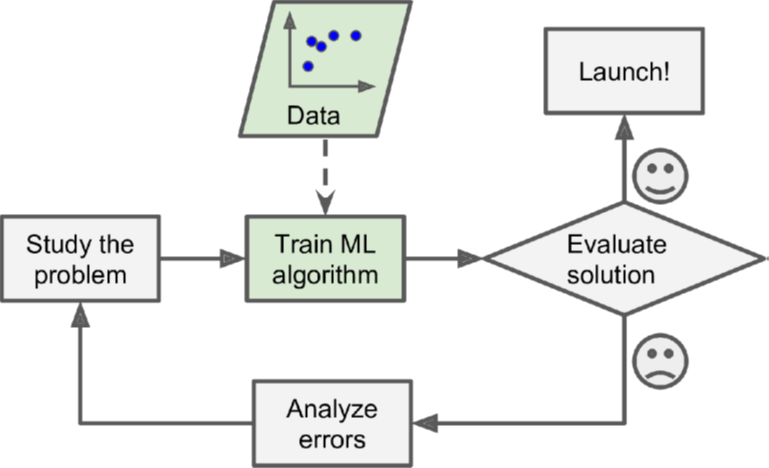
\includegraphics[width=1.0\linewidth]{images/ml.png} 
            \vspace{1em}
            \textit{The Machine Learning approach} \\
            % \vspace{0.5em}
            \textbf{Data + Answers = Rules}
        \end{column}
    \end{columns}
\end{frame}


\begin{frame}{Data Types}
    \begin{columns}[T]
        % --- Column 1: Structured Data ---
        \begin{column}{0.48\textwidth}
            \textbf{\large 1. Structured Data} \\
            \vspace{0.3em}
            \textit{Organized in rows and columns.}
            \vspace{0.8em}
            
            \begin{itemize}
                \setlength\itemsep{0.8em}
                \item \textbf{Tabular Data}
                \begin{itemize}
                    \item Spreadsheets, SQL Databases
                    \item \textit{Columns = Features, Rows = Samples}
                \end{itemize}
                \item \textbf{Time-Series Data}
                \begin{itemize}
                    \item Data indexed by time
                    \item Stock prices, Weather, IoT sensors
                \end{itemize}
            \end{itemize}
        \end{column}

        % --- Column 2: Unstructured Data ---
        \begin{column}{0.48\textwidth}
            \textbf{\large 2. Unstructured Data} \\
            \vspace{0.3em}
            \textit{Complex formats.}
            \vspace{0.8em}

            \begin{itemize}
                \setlength\itemsep{0.8em}
                \item \textbf{Text Data (NLP)}
                \begin{itemize}
                    \item Emails, Tweets, Documents
                \end{itemize}
                \item \textbf{Images \& Video (Computer Vision)}
                \begin{itemize}
                    \item Medical imaging, Surveillance, Face ID
                \end{itemize}
                \item \textbf{Audio Data}
                \begin{itemize}
                    \item Voice commands, Music processing
                \end{itemize}
            \end{itemize}
        \end{column}
    \end{columns}
    \textbf{Note:} \textit{Machine Learning excels at Structured Data, while Deep Learning dominates Unstructured Data.}
\end{frame}

\begin{frame}{Types of Machine Learning}
    \begin{block}{1. Supervised Learning}
        We have input data $X$ and corresponding target labels $y$.
        The goal is to learn a mapping $f(x) \approx y$.
    \end{block}
    \vspace{1em}

    \begin{columns}[T]
        % --- Regression ---
        \begin{column}{0.48\textwidth}
        \centering
            \textbf{\medium A. Regression} \\
            \textit{Predicting continuous values (e.g., Price)}
            \vspace{1em}
            \centering
            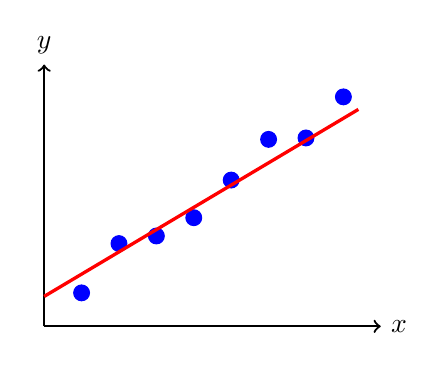
\begin{tikzpicture}[scale=0.95]
                % Axes
                \draw[->, thick] (0,0) -- (4.5,0) node[right] {$x$};
                \draw[->, thick] (0,0) -- (0,3.5) node[above] {$y$};
                % Data Points
                \foreach \x in {0.5,1,1.5,2,2.5,3,3.5,4} 
                    \filldraw [blue] (\x, 0.6*\x + 0.4 + 0.3*rand) circle (3pt);
                % Regression Line
                \draw [red, very thick] (0,0.4) -- (4.2,2.9);
            \end{tikzpicture}
        \end{column}

        % --- Classification ---
        \begin{column}{0.48\textwidth}
        \centering
            \textbf{\medium B. Classification} \\
            \textit{Predicting discrete categories (e.g., Spam Classification)}
            \vspace{1em}
            \centering
            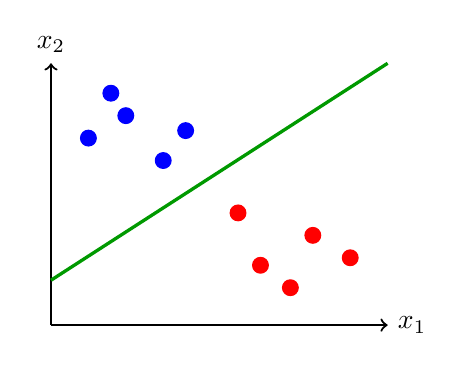
\begin{tikzpicture}[scale=0.95]
                % Axes
                \draw[->, thick] (0,0) -- (4.5,0) node[right] {$x_1$};
                \draw[->, thick] (0,0) -- (0,3.5) node[above] {$x_2$};
                % Class 0 (Blue Circles)
                \foreach \p in {(0.5,2.5), (1,2.8), (1.5,2.2), (0.8,3.1), (1.8,2.6)} 
                    \filldraw [blue] \p circle (3pt);
                % Class 1 (Red Squares - visually circles here for simplicity)
                \foreach \p in {(2.8,0.8), (3.5,1.2), (3.2,0.5), (4,0.9), (2.5,1.5)} 
                    \filldraw [red] \p circle (3pt);
                % Decision Boundary
                \draw [green!60!black, very thick] (0,0.6) -- (4.5,3.5);
            \end{tikzpicture}
        \end{column}
    \end{columns}
\end{frame}

\begin{frame}{Types of Machine Learning}
    \begin{block}{2. Unsupervised Learning}
        We only have input data $X$ (No labels). 
        The goal is to discover hidden structures or patterns.
    \end{block}
    \vspace{1em}

    \begin{columns}[T]
        % --- Clustering ---
        \begin{column}{0.48\textwidth}
        \centering
            \textbf{\medium A. Clustering (Grouping)} \\
            \textit{Grouping similar examples (e.g., customers segmentation)}
            \vspace{1em}
            \centering
            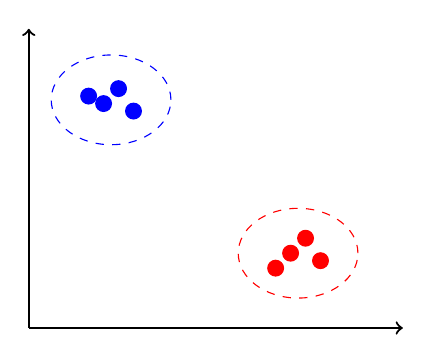
\begin{tikzpicture}[scale=0.95]
                % Fixed Axis Size for consistency
                \draw[->, thick] (0,0) -- (5,0);
                \draw[->, thick] (0,0) -- (0,4);
                
                % Cluster 1 (Top Left)
                \foreach \p in {(1,3), (1.2,3.2), (0.8,3.1), (1.4,2.9)} 
                    \filldraw [blue] \p circle (3pt);
                \draw [blue, dashed] (1.1,3.05) ellipse (0.8cm and 0.6cm);
                
                % Cluster 2 (Bottom Right)
                \foreach \p in {(3.5,1), (3.7,1.2), (3.3,0.8), (3.9,0.9)} 
                    \filldraw [red] \p circle (3pt);
                \draw [red, dashed] (3.6,1) ellipse (0.8cm and 0.6cm);
            \end{tikzpicture}
        \end{column}

        % --- Dimensionality Reduction ---
        \begin{column}{0.48\textwidth}
        \centering
            \textbf{\medium B. Dimensionality Reduction} \\
            \textit{Reduce the number of features (e.g., $100D \rightarrow 2D$ for visualization)}
            \vspace{1em}
            \centering
            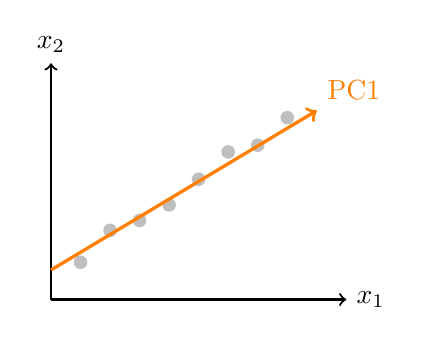
\begin{tikzpicture}[scale=0.75]
                % Fixed Axis Size for consistency
                \draw[->, thick] (0,0) -- (5,0) node[right] {$x_1$};
                \draw[->, thick] (0,0) -- (0,4) node[above] {$x_2$};
                
                % Data points roughly on a diagonal
                \foreach \x in {0.5, 1, 1.5, 2, 2.5, 3, 3.5, 4}
                    \filldraw [gray!50] (\x, 0.6*\x + 0.5 + 0.2*rand) circle (3pt);
                
                % PC1 Line
                \draw [orange, very thick, ->] (0,0.5) -- (4.5,3.2) node[above right] {PC1};
            \end{tikzpicture}
        \end{column}
    \end{columns}
\end{frame}

\begin{frame}{Types of Machine Learning}
    \begin{block}{3. Reinforcement Learning}
        Learning through trial and error. An \textbf{Agent} takes actions in an \textbf{Environment} to maximize cumulative \textbf{Reward}.
    \end{block}
    \vspace{1em}

\centering
    \begin{tikzpicture}[
        auto,
        node distance=4cm, % Increased distance for breathing room
        block/.style={
            rectangle, 
            draw, 
            text width=2.5cm, 
            text centered, 
            rounded corners, 
            minimum height=1.5cm,
            font=\large\bfseries
        },
        line/.style={draw, -{Latex[length=3mm]}, thick}
    ]
        % Nodes
        \node [block, fill=blue!10] (agent) {Agent};
        \node [block, fill=green!10, right=of agent] (env) {Environment};

        % Curved Arrows (The standard RL Loop look)
        \path [line] (agent) edge[bend left=30] node[above] {Action ($A_t$)} (env);
        \path [line] (env) edge[bend left=30] node[below] {State ($S_t$), Reward ($R_t$)} (agent);
        
    \end{tikzpicture}
    
    \vspace{1em}
    \begin{itemize}
        \item \textbf{Examples}: Chess engines (AlphaZero), Robot navigation, Stock trading bots, LLMs Preference Finetuning (RLHF).
    \end{itemize}
\end{frame}

\subsection{The Three Pillars of Learning}
